\section{eo\-Select\-From\-Worth$<$ EOT, Worth\-Type $>$ Class Template Reference}
\label{classeo_select_from_worth}\index{eoSelectFromWorth@{eoSelectFromWorth}}
selects one element from a population (is an {\bf eo\-Select\-One}{\rm (p.\,\pageref{classeo_select_one})}) but the selection is based on a std::vector of Worth that is different from the fitnesses (e.g.  


{\tt \#include $<$eo\-Select\-From\-Worth.h$>$}

Inheritance diagram for eo\-Select\-From\-Worth$<$ EOT, Worth\-Type $>$::\begin{figure}[H]
\begin{center}
\leavevmode
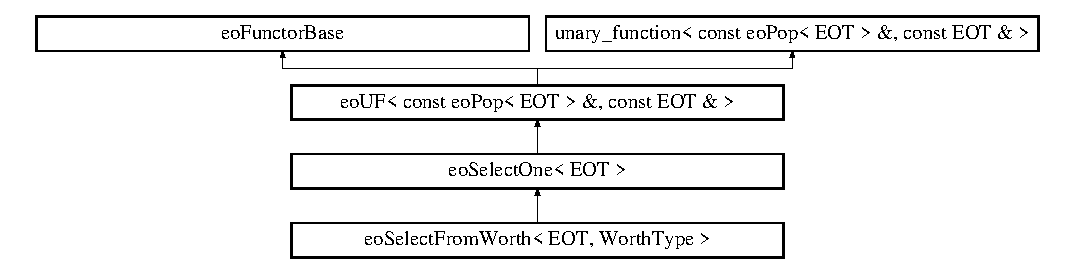
\includegraphics[height=3.23699cm]{classeo_select_from_worth}
\end{center}
\end{figure}
\subsection*{Public Member Functions}
\begin{CompactItemize}
\item 
{\bf eo\-Select\-From\-Worth} ({\bf eo\-Perf2Worth}$<$ {\bf EOT}, Worth\-Type $>$ \&\_\-perf2Worth)\label{classeo_select_from_worth_a0}

\item 
virtual void {\bf setup} (const {\bf eo\-Pop}$<$ {\bf EOT} $>$ \&pop)\label{classeo_select_from_worth_a1}

\begin{CompactList}\small\item\em virtual function to setup some population stats (for instance eo\-Proportional can benefit greatly from this) \item\end{CompactList}\end{CompactItemize}
\subsection*{Protected Member Functions}
\begin{CompactItemize}
\item 
void {\bf check\_\-sync} (unsigned index, const {\bf EOT} \&\_\-eo)\label{classeo_select_from_worth_b0}

\end{CompactItemize}
\subsection*{Protected Attributes}
\begin{CompactItemize}
\item 
{\bf eo\-Perf2Worth}$<$ {\bf EOT}, Worth\-Type $>$ \& {\bf perf2Worth}\label{classeo_select_from_worth_p0}

\item 
std::vector$<$ typename EOT::Fitness $>$ {\bf fitness}\label{classeo_select_from_worth_p1}

\end{CompactItemize}


\subsection{Detailed Description}
\subsubsection*{template$<$class EOT, class Worth\-Type = double$>$ class eo\-Select\-From\-Worth$<$ EOT, Worth\-Type $>$}

selects one element from a population (is an {\bf eo\-Select\-One}{\rm (p.\,\pageref{classeo_select_one})}) but the selection is based on a std::vector of Worth that is different from the fitnesses (e.g. 

{\bf EO}{\rm (p.\,\pageref{class_e_o})} fitness is what Koza terms \char`\"{}raw fitness\char`\"{}, Worth is what the selection is based upon).

see class {\bf eo\-Perf2Worth}{\rm (p.\,\pageref{classeo_perf2_worth})}: an {\bf eo\-Stat}{\rm (p.\,\pageref{classeo_stat})} that transforms fitnesses into Worthes

Note: Worthes will not always be doubles - see some multi-objective techniques where it is a std::pair of doubles ...

It has to have a $<$ operator it you want to call an existing selector (see selector.h) - but of course you can write the whole thing ... 



Definition at line 51 of file eo\-Select\-From\-Worth.h.

The documentation for this class was generated from the following file:\begin{CompactItemize}
\item 
eo\-Select\-From\-Worth.h\end{CompactItemize}
